% -*- mode:flyspell; mode:latex -*-
\documentclass[12pt]{article}

% \addtolength{\oddsidemargin} {-0.885in}
% \addtolength{\textwidth}{1.75in}
% \addtolength{\evensidemargin}{-0.8in}
% topmargin -0.5in
\usepackage[a4paper, top=1cm, left=1.5cm, right=1.5cm]{geometry} % width= , 

\usepackage[latin1]{inputenc}
\usepackage[T1]{fontenc}
\usepackage[english]{babel}
\usepackage{graphicx}
\usepackage{float}


\usepackage{tikz}
\usepackage{[caption}
\usetikzlibrary{arrows}
\usetikzlibrary{decorations.markings}
\usetikzlibrary{decorations.pathmorphing}
% \usepackage[absolute,overlay]{textpos}
% \usepackage{onimage}

\usepackage{times}
\usepackage{graphics}

% \usepackage{subfigure}
% \usepackage{scalefnt}
%
% \renewcommand\thesubfigure{\arabic{subfigure}}

\usepackage{amsmath}
\usepackage{hyperref}
\usepackage{hhline}
\usepackage{subfig}
\usepackage{color}
\usepackage[all]{hypcap}

\usepackage[normalem]{ulem}  % for striking out
% \usepackage{fancyhdr}
% \pagestyle{fancy}
% \fancyhead[C]{}
% \fancyhead[L] {\it{Mu2e-doc-29670-v1.0} }
%%%%%%%%%%%%%%%%%%%%%%%%%%%%%%%%%%%%%%%%%%%%%%%%%%%%%%%%%%%%%%%%%%%%%%%%%%%%%%
% use natbib - biblatex not available on Mu2e interactive nodes
%%%%%%%%%%%%%%%%%%%%%%%%%%%%%%%%%%%%%%%%%%%%%%%%%%%%%%%%%%%%%%%%%%%%%%%%%%%%%%
\usepackage[square,sort,comma,numbers]{natbib}

% location of the .bib files: env var BIBINPUTS (~/library/bibliography)

% \usepackage[backend=biber, style=numeric-comp, sorting=ynt] {biblatex}
% \addbibresource{clfv.bib}

% \addbibresource{stntuple.bib}
% \addbibresource{mu2e_web.bib}
% \addbibresource{radiative_pion_capture.bib}

\graphicspath{{figures/}}
%%%%%%%%%%%%%%%%%%%%%%%%%%%%%%%%%%%%%%%%%%%%%%%%%%%%%%%%%%%%%%%%%%%%%%%%%%%%%%
% for portability, make sure all commands are included locally
% order them alphabetically
%%%%%%%%%%%%%%%%%%%%%%%%%%%%%%%%%%%%%%%%%%%%%%%%%%%%%%%%%%%%%%%%%%%%%%%%%%%%%%
% \include{commands}

\newcommand {\keVc}       {\mbox{$\rm keV\!/\!c$}}
\newcommand {\kmax}       {\mbox{$k_{\rm max}$}}

\newcommand {\MeVc}       {\mbox{$\rm MeV\!/c$}}
\newcommand {\MeVcsq}     {\mbox{$\rm MeV\!/c^2$}}

\newcommand {\mumemconv}[1][A] {\mbox{$\mu^- \textrm{#1} \rightarrow e^- \textrm{#1}$}}
% Define a relay to have 2 default arguments instead of limit of 1
\newcommand {\mumepconv}[1][A] {%
  \def\ArgI{{#1}}%store the first argument
  \mumepconvRelay
}
\newcommand \mumepconvRelay[1][A]  {\mbox{$\mu^- \textrm{\ArgI} \rightarrow e^+ \textrm{#1}$}}
\newcommand {\muminus}    {\mbox{$\mu^-$}}
\newcommand {\muplus}    {\mbox{$\mu^+$}}
\newcommand {\MuToEm}     {\mbox{$\mu^- \ra e^-$}}
\newcommand {\MuToEp}     {\mbox{$\mu^- \ra e^+$}}
\newcommand {\MuPToEp}    {\mbox{$\mu^+ \ra e^+$}}
\newcommand {\ra}        {\rightarrow}
\newcommand {\tandip}    {\mbox{$\tan \lambda$}}

\newcommand {\Pb}[1]     {\mbox{$\rm ^{#1}Pb$}}                 % isotopes of lead
\newcommand {\Au}[1]     {\mbox{$\rm ^{#1}Au$}}                 % isotopes of gold
\newcommand {\Ir}[1]     {\mbox{$\rm ^{#1}Ir$}}                 % isotopes of iridium
%%%%%%%%%%%%%%%%%%%%%%%%%%%%%%%%%%%%%%%%%%%%%%%%%%%%%%%%%%%%%%%%%%%%%%%%%%%%%%
% editing commands
%%%%%%%%%%%%%%%%%%%%%%%%%%%%%%%%%%%%%%%%%%%%%%%%%%%%%%%%%%%%%%%%%%%%%%%%%%%%%%
\newcommand {\add}[1]    {{\red #1}}
\newcommand {\alt}[1]    {{\green #1}} %alternate comment color
\newcommand {\del}[1]    {{\blue \sout{#1}}}
\newcommand {\dlt}[1]    {{\violet \sout{#1}}} %alternate delete color

\newcommand {\black}     {\color{black}}
\newcommand {\red}       {\color{red}}
\newcommand {\blue}      {\color{blue}}
\newcommand {\strike}[1] {{\blue \sout{#1}}}
%%%%%%%%%%%%%%%%%%%%%%%%%%%%%%%%%%%%%%%%%%%%%%%%%%%%%%%%%%%%%%%%%%%%%%%%%%%%%%
\begin{document}

\begin{titlepage}
  \begin{flushright}
    \bf {MU2E/PHYSICS/xxxxx} \\
    version 1.0
    \today
 \end{flushright}

  \vspace{1cm}

  \begin{center}
    {\Large \bf Commissioning of the Mu2e Data AcQuisition system and the Vertical Slice Test of the straw tracker

      \vspace{0.3in}

      11. Mu2e ROC simulation
    }

    \vspace{1cm}
%     S. Gamba  \footnote{\texttt{Fermilab; e-mail:s.gamba2\@studenti.unipi.it} (University of Pisa)
%     P. Murat \footnote{\texttt{Fermilab; e-mail: murat\@fnal.gov} (FNAL)

   
    version 1.0
    \today
 \end{center}

  \begin{abstract}
    This note presents an analysis of data coming from the teststand of the motherboard and the comparison with ROC simulation.
    \vspace{0.2in}
  \end{abstract}

\end{titlepage}
% \frontmatter
% \chapter*{Abstract}
%
% \addcontentsline{toc}{chapter}{Abstract}
%
% \mainmatter
%
{\tableofcontents}

%%%%%%%%%%%%%%%%%%%%%%%%%%%%%%%%%%%%%%%%%%%%%%%%%%%%%%%%%%%%%%%%%%%%%%%%%%%%%%%
%\chapter{Calibration}
%%%%%%%%%%%%%%%%%%%%%%%%%%%%%%%%%%%%%%%%%%%%%%%%%%%%%%%%%%%%%%%%%%%%%%%%%%%%%%%
% \input{input_data}

%%%%%%%%%%%%%%%%%%%%%%%%%%%%%%%%%%%%%%%%%%%%%%%%%%%%%%%%%%%%%%%%%%%%%%%%%%%%%%%
\newpage
\section {Notes for the authors}
\subsection {Revision history} 
\begin{itemize}
\item
  v1.01: initial version
\end{itemize}

%%%%%%%%%%%%%%%%%%%%%%%%%%%%%%%%%%%%%%%%%%%%%%%%%%%%%%%%%%%%%%%%%%%%%%%%%%%%%%
\section {Introduction to the analysis}

In this note, we present an analysis of the data derived from the readout teststands of the motherboard.
This analysis was performed with the aim of characterizing the functionality of the Data Acquisition (DAQ) system.
A signal generator was employed to send pulses and we tried to understand the output and non-output of the DTC. 
Our study centered on testing the performance of ROCs and DTCs, actually we were reading 1 ROC (96 channels), 
which is the equivalent of one panel or 2 ROCs. The analysis was executed employing a single DTC.
During the analysis, we had the capability to change different generator's features. We varied the event
window duration between successive pulses and modulated the generator's operating frequency. 
Specifically, we could operate with two distinct frequencies: 31.29 MHz/(2$^7$+1), resulting in approximately 250 kHz,
and 31.29 MHz/(2$^9$+1), 60 kHz. \\
The selection of the event window duration and the frequency played an important role in determining the number of hits per event,
considering that the ROC buffer possessed a storage capacity for up to 255 hits. The relationship between the generator 
and readout counts can be summarized as follows:
\begin{itemize}
    \item $N_{gen} \ < \ $255: $N_{readout} \ = \ N_{gen}$;
    \item $N_{gen} \ \geq \ $255: $N_{readout} \ = \ 255$.
\end{itemize}

%%%%%%%%%%%%%%%%%%%%%%%%%%%%%%%%%%%%%%%%%%%%%%%%%%%%%%%%%%%%%%%%%%%%%%%%%%%%%%
\section{Time distribution}
The analysis started the data time distribution 
After a preliminary observation of the data time distribution, as illustrated in Fig. \ref{fig:1}, the initial though  was 
the occurrence of a cessation in data acquisition for specific channels at a certain time.

\begin{figure}[H]
  \hspace{-0.5in}
  \begin{tikzpicture}
    \node[anchor=south west,inner sep=0] at (0,0.) {
      % \node[shift={(0 cm,0.cm)},inner sep=0,rotate={90}] at (0,0) {}
      % \makebox[\textwidth][c] {
      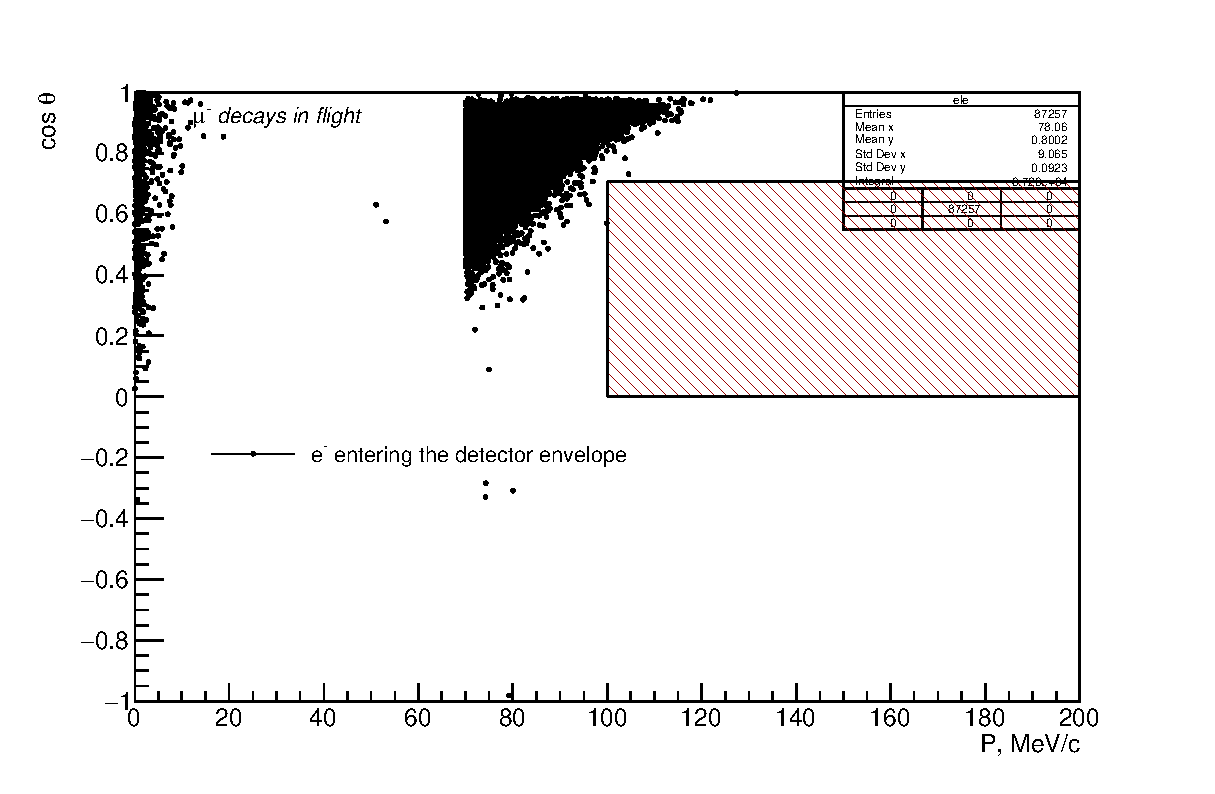
\includegraphics[width=0.5\textwidth]{figures/pdf/figure_04000_bmum0s5bb0_spmc_1_cth_vs_mom}
      % }
    };
    \node[anchor=south west,inner sep=0] at (10,0.) {
      % \node[shift={(0 cm,0.cm)},inner sep=0,rotate={90}] at (0,0) {}
      % \makebox[\textwidth][c] {
      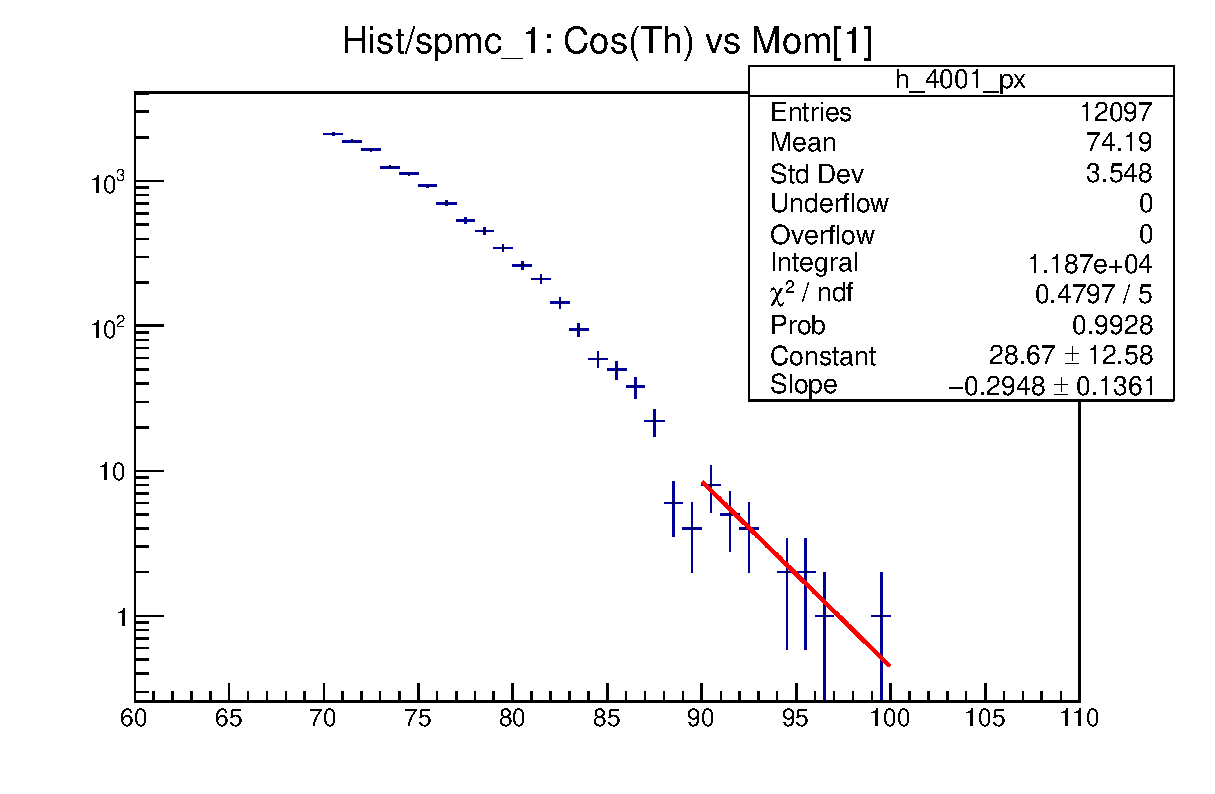
\includegraphics[width=0.5\textwidth]{figures/pdf/figure_04001_bmum0s5bb0_spmc_1_cth_vs_mom}
      % }
    };
  \end{tikzpicture}
  \caption{
    \label{fig:1}
    Electrons from muon decays downstream VD9 entering the detector envelope
  }
\end{figure}
At this point we have plotted the number of hits versus the channel number in the order that we expected, as we can see in Fig. \ref{fig:2}.

\begin{figure}[H]
      \includegraphics[width=0.6\textwidth]{figures/pdf/figure_03700_bmum0s37b0_vdet_xx09_mom}
  \caption{
    \label{fig:2}
    Left: momentum distributions of particles reaching VD9;
    Right: momentum distributions at VD9 of particles stopped in the stopping target
  }
\end{figure}
We thought it was necessary to characterize the apparatus with a Monte Carlo simulation for our Data Acquisition (DAQ) system, in order to understand the interruptions.

\section {Datasets}

The results presented in this note are based on the analysis of the \muminus\ beam {\bf bmum0}
family of SU2020 datasets \cite{SU2020_DATASETS}, resimulated with the increased statistics
of $1\times 10^9$ protons on target. The family includes the following datasets: 

\begin{itemize}
\item
  bmum0s11b0: output of Stage1 simulation: muons produced in pA interactions at the production target are
  traced to the plane in front of the TS31 collimator
\item
  bmum0s21b0: output of Stage1 simulation traced to the plane in front of TS5 collimator
\item
  bmum0s36b0: events with $p ~>~ 100 \MeVc$ electrons produced at Stage1 traced up to VD9
  (virtual detector in front of the stopping target)
\item
  bmum0s37b0: (bmum0s27b0-bmum0s28b0) events traced up to VD9.
  Those are events without $p ~>~ 100 \MeVc$ electrons in the end of Stage2
\item
  bmum0s38b0: events with $p ~>~ 100 \MeVc$ electrons produced at Stage2 traced up to VD9
\item
  bmum0s39b0: strip from bmum0s37b0, events with  $p ~>~ 100 \MeVc$ electrons produced in TS5 and
  in the DS before the stopping target
\item
  bmum0s3ab0: strip from bmum0s37b0. Event withs $p ~>~ 100 \MeVc$ negative muon at VD9.
  The dataset used to estimate background from muon scattering in the stopping target
\item
  bmum0s3ab0: strip from bmum0s37b0. Event withs $p ~>~ 100 \MeVc$ negative muon at VD9.
  The dataset used to estimate background from muon scattering in the stopping target
\item
  bmum0s47b0: (bmum0s37b0 - bmum0s39b0) traced to VD10, virtual detector right after the stopping target.
  Those are events which didn't have  $p ~>~ 100 \MeVc$ at VD9
\item
  bmum0s4bb0: strip from bmum0s47b0. Events with $p ~>~ 70 \MeVc$ mu- P>70 MeV/c at VD10.
  The dataset used to estimate background from muon decays in flight.
\item
  bmum0s56b0: bmum0s36b0 traced through DS, selection of events with $p ~>~ 100 \MeVc$ electron entering
  the detector (tracker+calorimeter) envelope volume. Resampling factor of 10,000
\item
  bmum0s58b0: bmum0s36b0 traced through DS, selection of events with $p ~>~ 100 \MeVc$ electron entering
  the detector (tracker+calorimeter) envelope volume. Resampling factor of 10,000
\item
  bmum0s59b0: bmum0s36b0 traced through DS, selection of events with $p ~>~ 100 \MeVc$ electron entering
  the detector (tracker+calorimeter) envelope volume. Resampling factor of 10,000
\item
  bmum0s5ab0: bmum0s3ab0 traced through DS, selection of events with a $p ~>~ 100 \MeVc$ muon
  entering the detector envelope volume. Resampling factor of 10,000
\item
  bmum0s5bb0: bmum0s4bb0 traced through DS, selection of events with a $p ~>~ 100 \MeVc$ electron
  entering the detector envelope volume. Resampling factor of 1,000.
\end{itemize}

%%%%%%%%%%%%%%%%%%%%%%%%%%%%%%%%%%%%%%%%%%%%%%%%%%%%%%%%%%%%%%%%%%%%%%%%%%%%%%
\section {Momentum distributions of the beam particles }


\begin{figure}[H]
  \hspace{-0.5in}
  \begin{tikzpicture}
    \node[anchor=south west,inner sep=0] at (0,0.) {
      % \node[shift={(0 cm,0.cm)},inner sep=0,rotate={90}] at (0,0) {}
      % \makebox[\textwidth][c] {
      \includegraphics[width=0.6\textwidth]{figures/pdf/figure_03700_bmum0s37b0_vdet_xx09_mom}
      % }
    };
    \node[anchor=south west,inner sep=0] at (10,0.) {
      % \node[shift={(0 cm,0.cm)},inner sep=0,rotate={90}] at (0,0) {}
      % \makebox[\textwidth][c] {
      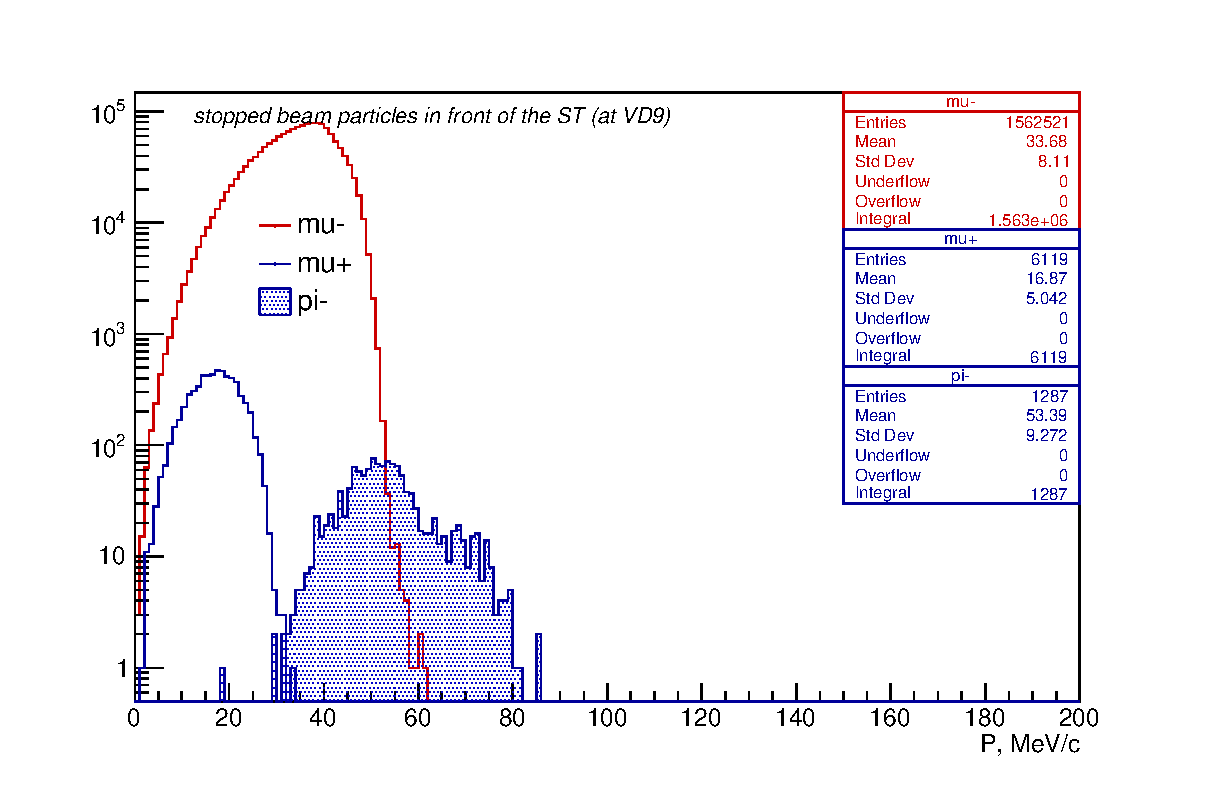
\includegraphics[width=0.6\textwidth]{figures/pdf/figure_03100_bmum0s31b0_vdet_xx09_mom}
      % }
    };
  \end{tikzpicture}
  \caption{
    \label{fig:03700_bmum0s37b0_vdet_xx09_mom}
    Left: momentum distributions of particles reaching VD9;
    Right: momentum distributions at VD9 of particles stopped in the stopping target
  }
\end{figure}

%%%%%%%%%%%%%%%%%%%%%%%%%%%%%%%%%%%%%%%%%%%%%%%%%%%%%%%%%%%%%%%%%%%%%%%%%%%%%%

\section {Beam electrons}

%%%%%%%%%%%%%%%%%%%%%%%%%%%%%%%%%%%%%%%%%%%%%%%%%%%%%%%%%%%%%%%%%%%%%%%%%%%%%% 
\subsection {Electrons Entering the Detector Envelope}


%%%%%%%%%%%%%%%%%%%%%%%%%%%%%%%%%%%%%%%%%%%%%%%%%%%%%%%%%%%%%%%%%%%%%%%%%%%%%%
\newpage
\section{Summary}
Upper bounds on the direct beam-related backgrounds are as follows:
\begin{itemize}
\item
  background from beam electrons scattered in the stopping target < $1 \times 10^{-3}$
\item
  background from muon decay in flights < $1 \times 10^{-3}$
\item
  background from beam muons scattered in the stopping target < $1 \times 10^{-5}$
\end{itemize}
%%%%%%%%%%%%%%%%%%%%%%%%%%%%%%%%%%%%%%%%%%%%%%%%%%%%%%%%%%%%%%%%%%%%%%%%%%%%%%
%
%%%%%%%%%%%%%%%%%%%%%%%%%%%%%%%%%%%%%%%%%%%%%%%%%%%%%%%%%%%%%%%%%%%%%%%%%%%%%%
\newpage
\bibliographystyle{unsrtnat}
\bibliography{local,clfv,dio,mu2e_internal_notes}

\end{document}

%%%%%%%%%%%%%%%%%%%%%%%%%%%%%%%%%%%%%%%%%%%%%%%%%%%%%%%%%%%%%%%%%%%%%%%%%%%%%%
% small font sizes: \small \footnotesize \scriptsize \tiny
% ------------------------------------------------------------------------------
% templates
% ------------------------------------------------------------------------------
% Table ~\ref{table:summary} gives summary the numbers used in this study.
%
% \hspace{-0.1in}
% \begin{table}[htbp]
%   \label{table:summary}
%   \begin{center}
%     {\renewcommand{\arraystretch}{1.0}   % change 1.0 to 1.1 to increase the spacing between the table lines
%       \begin{tabular}{|c|c|c|c|}
%         \hline
%                             & default TS geometry & misaligned TS geometry   &  Ratio(default/misaligned)    \\
%         \hline
%         $N_{POT}$            &  $4.96 \cdot 10^6$  &    $5.00 \cdot 10^6$      &   0.992   \\
%         $N_{\mu}^{TS3u}$      &  65648              &     61354                 &   1.070   \\
%         $N_{\mu}^{TS5}$       &  28517              &     27351                 &   1.043   \\
%         $N_{\mu}^{ST}$        &  8868               &      8396                 &   1.056   \\
%         $N_{\mu}^{ST}/N_{POT}$ &  $1.79 \pm 0.02$    &    $1.68 \pm 0.02$        &   $1.065 \pm 0.03$        \\
%         \hline
%       \end{tabular}
%     }
%   \end{center}
%   \caption{
%     Muons rates at different points of the Mu2e beamline and stopping muon rates for nominal and
%     misaligned TS geometries
%   }
%   % \vspace{0.5in}
% \end{table}
